\section{Ontologies as Prior Knowledge in GUHA Mining} \label{OntologiesAssociation}

\subsection{The GUHA Method}
\label{section:guha}
The GUHA method, developed in the mid-sixties, is one of the first methods of exploratory data analysis. 
It is a general framework for retrieving interesting knowledge from data. 
The method has solid theoretical foundations based on observational calculi and statistics \cite{GUHA}. 
For the purposes of this paper, let us only explain the basic principles of the method, as shown in Figure \ref{fig:GUHA}.

\begin{figure}[ht]
\centering
\mbox{\resizebox{60mm}{!}{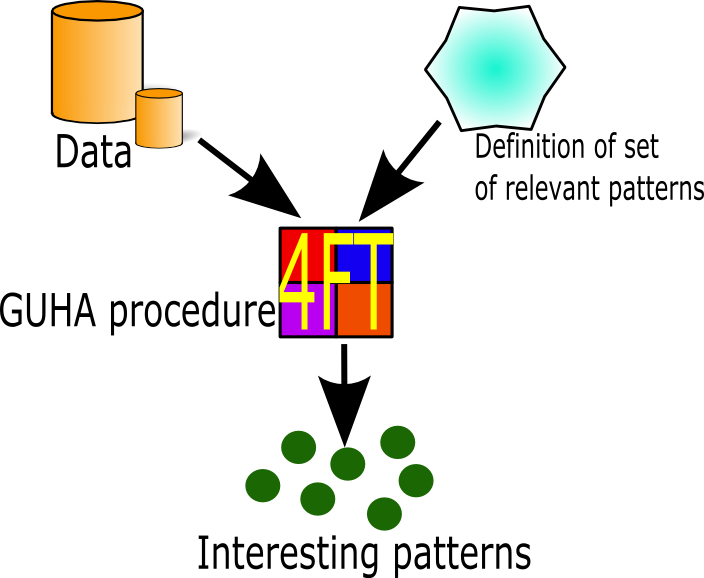
\includegraphics{GUHA.png}}}
\caption{The GUHA method}
\label{fig:GUHA}
\end{figure}

The GUHA method is realized by GUHA procedures such as the 4FT procedure (used in our work), located in the middle of the figure. 
Inputs of the procedure are the data and a simple definition of a possibly large set of relevant patterns. 
The procedure automatically generates all relevant patterns and verifies them against the source data. 
Patterns that are positively verified are output by the procedure.

Although GUHA is not in principle restricted to mining association rules, the most frequently used GUHA procedures mine for \emph{generalized association rules} as defined in \cite{Rauch}. 
The association rules are generalized in two ways: they allow a more complex structure in antecedent and consequent, and also allow for a wide variety of relations (quantifiers) between antecedent and consequent to be examined. 
A detailed comparison study between the `mainstream' association mining and association mining using GUHA can be found in \cite{HajekHolena}.

%\subsection{Domain Ontologies for Data Mining}

%Domain ontologies describe abstract knowledge about a certain domain. On the other hand exploratory data mining methods (such as the GUHA method) aim to retrieve unknown knowledge from data of a given domain. Therefore ontologies should be used in order to enhance the data mining process.

%In \cite{Ontology} authors identified four stages of association mining process (corresponding to the CRISP-DM cycle) that are likely to benefit from ontological knowledge: data understanding, task design, result interpretation and result dissemination over the semantic web. Experiments showing usability were carried out with 4ft-Miner, one of the GUHA procedures. 

%This work is continuation of \cite{Ontology}. One of the weaknesses of \cite{Ontology} absence of working tool for automation of ontology usage in KDD, majority of experiments was done by hand. We decided further research to be carried out in this direction. In \cite{Ralbovsky} detailed analysis of possibilities of ontology usage automation was accomplished. It was found that the most promising data preparation is the most promising stage for automation. 

\subsection{Using Domain Ontologies in Data Preparation for GUHA}
\label{OntologiesDataPrep}

Previous research \cite{Cespivova,Ralbovsky} proposed numerous potential ways to enhance the (GUHA-based) KDD process using ontologies. 
Based on these initial studies, we identified two ways of ontology usage that looked most promising. 
These are:
\begin{itemize}
	\item Construction of adequate attribute categorization with the aid of ontologies
	\item Identification and exploitation of semantically related attributes
\end{itemize}

\subsubsection{Construction of Attribute Categories.}

Data mining tools often deal with data for which some kind of higher-level semantics could be assigned to individual values.
For example, for blood pressure there are predefined values that divide the domain in a meaningful way: say, blood pressure above 140/90 mm Hg is considered as hypertension. 
Without proper categorization, data mining may give opaque or even misleading results.
%We think that proper categorization of data is crucial for successful data preparation phase. 

Therefore, a way of storing the categorization information in an OWL ontology has been proposed, and tools for automatic creation of categorized attributes was implemented in the Ferda tool. 
Section~\ref{OntologiesFerda} describes details.

\subsubsection{Identification and Exploitation of Semantically Related Attributes.}

Examined data matrices often consist of a large number of columns representing information about real-world entities. 
These entities are often semantically close to each other, such relationships may however not be always be transferred to the data mining phase.
Ontologies have representational power to express various kinds of semantic closeness, foremost within the class taxonomy. 
Identification of mutually related entities can be exploited so as to meaningfully arrange the corresponding data attributes in the examined matrix (in the data preparation phase) or to construct meaningful data mining tasks (in the modelling phase). 

We implemented a mechanism that identifies semantically related attributes in data and prepares them for further usage. 
Details are again in section~\ref{OntologiesFerda}.

%In previous works \cite{Cespivova,Ralbovsky} the usage of ontologies during KDD process was exploring. There were identified and specified concrete ways of using ontologies. \cite{Zeman} continued in the research and identified the most promising ways of ontology usage. They are:
%\begin{itemize}
%	\item Creation of attributes with aid of ontologies
%	\item Identification and usage of related attributes
%\end{itemize}

%Creation of attributes with aid of ontologies.

%The goal of this way of usage is is to create an attribute from a datatable column. This means to divide values of the column into categories which will be then an inputs for GUHA procedures. An example for better understanding: we have datatable column systolic blood pressure. The column is stored in a database and has an integer type. There is a plenty of possibilities how to categorize this column, but there is one, which is better than the others. In medical field, there are explicitly specified values which identifies whether the pressure is high, low, etc. These values are widely familiar to people from medical field and the knowledge of it is shared among all these people. From this point of view, this kind of knowledge is very similar to knowledge saved in ontologies (see definition of Ontology: Ontology is a formal specification of a shared conceptualization).

%Main idea of this way of usage is to understand the semantics of the data, which could help us work with it. For that we need to store somewhere the knowledge about the semantics and we need to link data with the correct semantics. Work \cite{Zeman} describes in detail how it is possible to achieve that and implements this way of ontology usage. The task can be divided into two parts.
%\begin{enumerate}
%	\item Definition of information which is useful to describe a semantics of entities.
%	\item Way of connecting particular data with the semantics.
%\end{enumerate}

%\cite{Ralbovsky} offers first draft of information, which can help us recognize how to deal with %data. \cite{Zeman} thinks more thoroughly about the information and offers an updated list, which %is easy to understand by computers (easy to use for algorithms) as well as by people. Specified %information are: 
%\begin{itemize}
%	\item cardinality - it specifies the semantics of the entity, especially it says wheter it is reasonable to compare two values of the dataset. There are 4 enumerate values for cardinality:	
%		\begin{itemize}
%			\item Cardinal - the dataset where is a scale is defined. It makes sense to compare two values from the dataset and one of them is greater than the other one or they are same. In addition at cardinal sets there is also defined a difference between two values. One can evaluate how far the values are from each other.
%			\item Ordinal - similar to Cardinal but without a difference defined. 
%			\item Ordinal Cyclic - there is defined scale but the values are repeating in a cycling way. E.g. days in a week: Monday is before Tuesday but concrete instance of the days doesn't have to be in the same order.
%			\item Nominal - it does not make sense to compare distinct values of the set.
%		\end{itemize}
%	\item minimum - minimum specifies the lowest possible value of an entity (it makes sense only at Cardinal or Ordinal values).
%	\item maximum - maximum specifies the highest possible value of an entity (it makes sense only at Cardinal or Ordinal values).
%	\item domain dividing values - they make sense only at Cardinal or Ordinal values and these are values which divide the domain.
%	\item significant values - significant values are values which are somehow special, e.g. typical values, extreme values etc.
%\end{itemize}

%Way of connecting particular data with the semantics.

%Although the advantage is not visible on first sight as we have to fill the ontology with additional info first and then we can use it. The main benefit is in reusability of ontologies and reusability of the mapping (e.g. more people work upon one database so one of them prepare mapping and others will simply use it).